\chapter{La respiration cellulaire et la fermentation}\label{ch:g12:respiration-fermentation}

Les muscles d'un coureur de marathon dépensent, en trois heures et
demie, environ une demi-mole d'\omterm{def:g12:respiration-fermentation:atp}{ATP} par minute --- un quart de
kilogramme de la molécule, fabriquée, utilisée et refabriquée des
milliers de fois à partir d'un stock qui durerait cinq secondes.
Chacune de ces molécules d'\omterm{def:g12:respiration-fermentation:atp}{ATP} est payée par un glucose ou un acide
gras démonté atome par atome, et par une molécule d'oxygène inspirée
au début et rejetée sous forme d'eau à la fin. Le
\cref{ch:g10:cell-metabolism} en a donné le bilan~; ce chapitre ouvre
la \omterm{def:g10:cells-common-unit:organelle}{mitochondrie} et suit le glucose à travers les trois étapes qui
convertissent son énergie en \omterm{def:g12:respiration-fermentation:atp}{ATP} --- et montre ce que fait une \omterm{def:g10:cells-common-unit:cell}{cellule}
quand l'oxygène vient à manquer.

\section{L'ATP, la monnaie}

\begin{definition}[ATP]\label{def:g12:respiration-fermentation:atp}
L'\emph{ATP}\index{ATP} (adénosine triphosphate) est un \omterm{def:g10:universal-dna:nucleotide}{nucléotide}
portant trois groupements phosphate à la file. Retirer le dernier
libère environ \qty{30}{kJ} par mole dans les conditions de la
\omterm{def:g10:cells-common-unit:cell}{cellule}, et tout processus cellulaire qui exige de
l'énergie --- contraction, transport, synthèse, la lumière d'une
luciole --- est entraîné par ce retrait. Le produit, l'ADP, est
rechargé en ATP par les réactions de ce chapitre. Une \omterm{def:g10:cells-common-unit:cell}{cellule} ne
détient que quelques secondes d'ATP et le renouvelle sans cesse~; un
humain au repos en recycle chaque jour à peu près l'équivalent de sa
propre masse corporelle.
\end{definition}

\begin{proposition}[Où se trouve l'énergie]\label{prop:g12:respiration-fermentation:oxidation}
Le glucose emmagasine de l'énergie dans ses liaisons
carbone--hydrogène~; la libérer, c'est transférer l'hydrogène, avec
ses électrons, à l'oxygène --- oxyder le glucose en dioxyde de carbone
et réduire l'oxygène en eau. Faite en une seule étape, comme dans une
flamme, l'opération laisserait partir l'énergie en chaleur. La \omterm{def:g10:cells-common-unit:cell}{cellule}
la mène en des dizaines de petites étapes, chacune conduite par une
\omterm{def:g11:enzymes-and-phenotype:enzyme}{enzyme}, et capte une part de l'énergie à plusieurs d'entre elles~:
l'hydrogène est d'abord chargé sur des molécules
transporteuses --- le \emph{NAD réduit} --- et n'est remis à l'oxygène
qu'à la fin.
\end{proposition}
\admitted

\section{Trois étapes}

\begin{proposition}[La glycolyse]\label{prop:g12:respiration-fermentation:glycolysis}
Dans le \omterm{def:g10:cells-common-unit:cell}{cytoplasme}, sans oxygène, un glucose (six carbones) est scindé
en deux molécules de \emph{pyruvate} (trois carbones chacune) par dix
étapes enzymatiques~: c'est la \emph{glycolyse}\index{glycolyse}. Le
bilan~: deux \omterm{def:g12:respiration-fermentation:atp}{ATP} consommés pour amorcer, quatre produits, soit un gain
net de 2 \omterm{def:g12:respiration-fermentation:atp}{ATP}, et deux NAD réduits chargés d'hydrogène. Le pyruvate
détient encore l'essentiel de l'énergie du glucose.
\end{proposition}
\admitted

\begin{proposition}[La mitochondrie achève l'oxydation]\label{prop:g12:respiration-fermentation:mitochondrion}
Quand l'oxygène est disponible, le pyruvate entre dans la
\emph{mitochondrie}\index{mitochondrie}, un \omterm{def:g10:cells-common-unit:organelle}{organite} limité par deux
membranes, l'interne étant repliée en \emph{crêtes} qui enferment un
liquide, la \emph{matrice}.
\begin{itemize}
  \item Dans la matrice, chaque pyruvate est démonté par un cycle de
        réactions, le \emph{cycle de Krebs}\index{cycle de Krebs}~:
        ses trois carbones s'en vont en trois $\mathrm{CO_2}$, son
        hydrogène est chargé sur des transporteurs (le NAD réduit et
        un second transporteur), et un peu d'\omterm{def:g12:respiration-fermentation:atp}{ATP} est fabriqué
        directement --- un par pyruvate.
  \item Dans la membrane interne, les transporteurs chargés remettent
        leurs électrons à une chaîne de \omterm{def:g10:chemistry-of-life:families}{protéines}, la \emph{chaîne
        respiratoire}, qui les fait descendre jusqu'à l'oxygène,
        lequel s'unit à des protons pour former de l'eau. L'énergie
        libérée le long de la chaîne pompe des protons à travers la
        membrane, et leur retour par une \omterm{def:g11:enzymes-and-phenotype:enzyme}{enzyme} rotative entraîne la
        synthèse d'\omterm{def:g12:respiration-fermentation:atp}{ATP} --- environ 26 par glucose.
\end{itemize}
Total pour un glucose~: environ 30 \omterm{def:g12:respiration-fermentation:atp}{ATP} (2 de la \omterm{prop:g12:respiration-fermentation:glycolysis}{glycolyse}, 2 du cycle,
quelque 26 de la chaîne), six $\mathrm{CO_2}$ libérés, six
$\mathrm{O_2}$ consommés, et le reste des \qty{2870}{kJ} en chaleur.
\end{proposition}
\begin{proof}[Preuves]
Des \omterm{def:g10:cells-common-unit:organelle}{mitochondries} isolées dans une enceinte close munie d'une sonde à
oxygène ne consomment pas d'oxygène lorsqu'on leur donne du glucose,
mais en consomment rapidement lorsqu'on leur donne du
pyruvate --- la \omterm{def:g10:cells-common-unit:organelle}{mitochondrie} ne peut pas partir du glucose~; c'est au
\omterm{def:g10:cells-common-unit:cell}{cytoplasme} de le faire. L'ajout d'un poison de la chaîne respiratoire
(le cyanure) arrête aussitôt la consommation, quel que soit le
\omterm{def:g11:enzymes-and-phenotype:enzyme}{substrat} présent. L'ajout d'ADP accélère la consommation et son
épuisement la ralentit~: l'usage de l'oxygène est couplé à la synthèse
d'\omterm{def:g12:respiration-fermentation:atp}{ATP}. Et les \omterm{def:g10:cells-common-unit:organelle}{mitochondries} du muscle de vol d'un colibri ou de la
cuisse d'un coureur de marathon ont des crêtes plusieurs fois plus
serrées que celles d'un tissu au repos.
\end{proof}

\begin{omfigure}
\begin{tikzpicture}
  \node[anchor=south west, inner sep=0] (img) at (0,0)
    {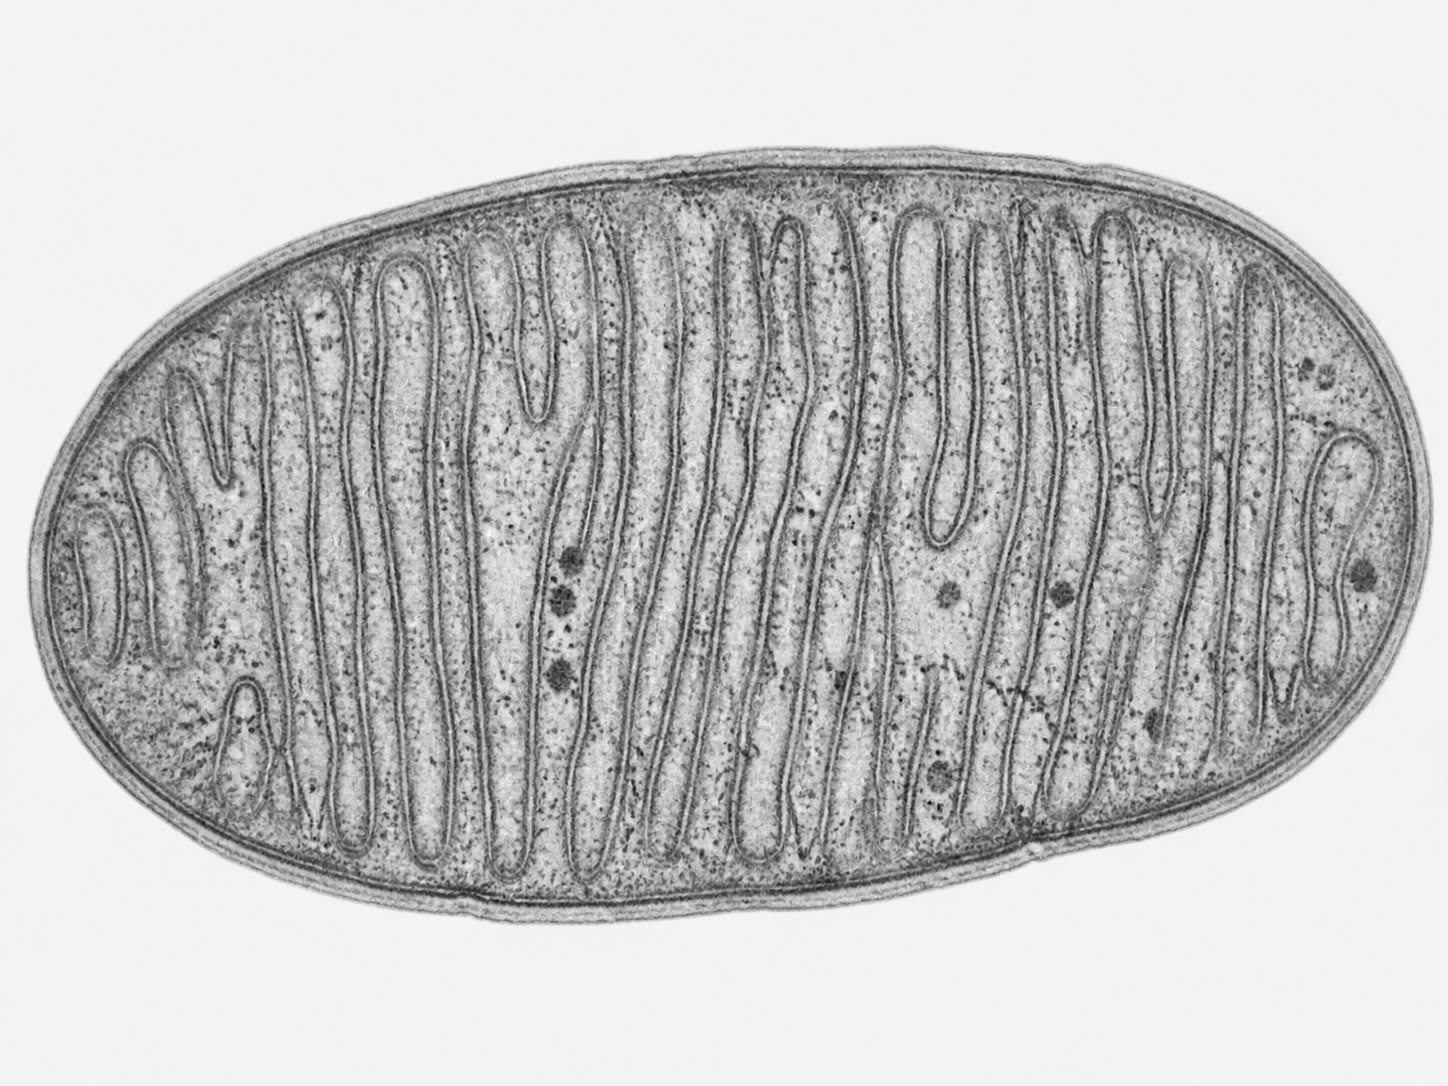
\includegraphics[width=0.5\linewidth]{images/book2/ai/g12-resp-mitochondrion-tem.jpg}};
  \begin{scope}[x={(img.south east)}, y={(img.north west)},
      every node/.style={font=\small}]
    \draw[omDef, thick] (0.08,0.55) -- (-0.04,0.80) node[left, align=right] {membrane\\ externe};
    \draw[omDef, thick] (0.20,0.45) -- (-0.04,0.25) node[left, align=right] {membrane interne,\\ repliée en crêtes};
    \draw[omDef, thick] (0.55,0.50) -- (0.55,-0.06) node[below] {matrice (cycle de Krebs)};
    \draw[omDef, thick] (0.80,0.60) -- (1.04,0.80) node[right, align=left] {crêtes~: la chaîne\\ respiratoire};
  \end{scope}
\end{tikzpicture}

{\small Une \omterm{def:g10:cells-common-unit:organelle}{mitochondrie} au microscope électronique. La membrane
interne est repliée en crêtes, qui portent la chaîne respiratoire et
l'\omterm{def:g11:enzymes-and-phenotype:enzyme}{enzyme} qui fabrique l'\omterm{def:g12:respiration-fermentation:atp}{ATP}~; le liquide qu'elles enferment, la
matrice, fait tourner le \omterm{prop:g12:respiration-fermentation:mitochondrion}{cycle de Krebs}.}
\end{omfigure}

\begin{omfigure}
\begin{tikzpicture}[font=\small, >=Stealth,
  b/.style={draw, rounded corners, align=center, minimum height=0.9cm}]
  % cytoplasm region
  \node[b, fill=omDef!8, minimum width=6.0cm, minimum height=6.2cm] (cyt) at (0,0) {};
  \node[anchor=north, font=\small\bfseries] at (cyt.north) {cytoplasme};
  \node[b, fill=omMeth!20, text width=2.4cm] (glu) at (0,2.0) {glucose (6 C)};
  \node[b, fill=omProp!20, text width=2.4cm] (pyr) at (0,-0.2) {2 pyruvates\\ (3 C chacun)};
  \draw[->, thick] (glu) -- node[right, align=left, font=\scriptsize] {glycolyse~:\\ $+2$ ATP, $+2$ NADH} (pyr);
  \node[b, fill=omThm!15, text width=2.6cm] (ferm) at (0,-2.4) {fermentation~:\\ lactate, ou\\ éthanol $+ \mathrm{CO_2}$};
  \draw[->, thick, omThm] (pyr) -- node[right, font=\scriptsize, align=left] {sans $\mathrm{O_2}$~:\\ NADH régénéré} (ferm);
  % mitochondrion region
  \node[b, fill=omProp!8, minimum width=6.4cm, minimum height=6.2cm, rounded corners=14pt] (mit) at (7.3,0) {};
  \node[anchor=north, font=\small\bfseries] at (mit.north) {mitochondrie};
  \node[b, fill=omProp!20, text width=2.6cm] (krebs) at (7.3,1.4) {cycle de Krebs\\ (matrice)~:\\ $6\,\mathrm{CO_2}$ sortent,\\ $+2$ ATP, transporteurs chargés};
  \node[b, fill=omThm!15, text width=2.8cm] (chain) at (7.3,-1.5) {chaîne respiratoire\\ (membrane interne)~:\\ transporteurs $+ \mathrm{O_2} \to \mathrm{H_2O}$,\\ $+26$ ATP};
  \draw[->, thick] (pyr.east) -- node[pos=0.72, above, font=\scriptsize] {avec $\mathrm{O_2}$} (krebs.west |- pyr.east);
  \draw[->, thick] (krebs) -- node[right, font=\scriptsize] {NAD réduit} (chain);
  \draw[->, thick] (10.9,-1.1) -- (chain.east |- 0,-1.1) node[pos=0, right] {$6\,\mathrm{O_2}$};
  \draw[->, thick] (chain.east |- 0,-1.9) -- (10.9,-1.9) node[right] {$6\,\mathrm{H_2O}$};
  \draw[->, thick] (krebs.east |- 0,1.8) -- (10.9,1.8) node[right] {$6\,\mathrm{CO_2}$};
\end{tikzpicture}

{\small Les trois étapes de la respiration, et le raccourci de la
\omterm{def:g10:cell-metabolism:fermentation}{fermentation}. La \omterm{prop:g12:respiration-fermentation:glycolysis}{glycolyse}, dans le \omterm{def:g10:cells-common-unit:cell}{cytoplasme}, donne deux \omterm{def:g12:respiration-fermentation:atp}{ATP} et deux
pyruvates~; dans la \omterm{def:g10:cells-common-unit:organelle}{mitochondrie}, le \omterm{prop:g12:respiration-fermentation:mitochondrion}{cycle de Krebs} les réduit à du
dioxyde de carbone et charge les transporteurs, que la chaîne
respiratoire décharge sur l'oxygène en fabriquant l'essentiel de
l'\omterm{def:g12:respiration-fermentation:atp}{ATP}. Sans oxygène, le pyruvate est dévié vers la \omterm{def:g10:cell-metabolism:fermentation}{fermentation}, qui
ne rapporte rien de plus.}
\end{omfigure}

\begin{example}[Lire un tracé d'oxygène]\label{ex:g12:respiration-fermentation:trace}
Des \omterm{def:g10:cells-common-unit:organelle}{mitochondries} isolées dans l'enceinte~: l'oxygène reste à
\qty{8}{mg/L}~; on ajoute du glucose, rien~; on ajoute du pyruvate,
l'oxygène baisse de \qty{0.5}{mg/L} par minute~; on ajoute de l'ADP,
la baisse s'accentue jusqu'à \qty{1.5}{mg/L} par minute pendant un
temps, puis revient à \num{0.5}~; on ajoute du cyanure, la baisse
s'arrête. Quatre faits en un seul tracé~: la \omterm{def:g10:cells-common-unit:organelle}{mitochondrie} a besoin de
pyruvate, non de glucose~; l'usage de l'oxygène est couplé à la
synthèse d'\omterm{def:g12:respiration-fermentation:atp}{ATP}~; ce couplage passe par la chaîne que bloque le
cyanure~; et une \omterm{def:g10:cells-common-unit:organelle}{mitochondrie} sans travail à faire tourne au ralenti.
\end{example}

\begin{omfigure}
\begin{tikzpicture}
\begin{axis}[
  width=0.9\linewidth, height=5.6cm,
  axis x line=bottom, axis y line=left,
  xmin=0, xmax=16, ymin=0, ymax=10,
  xlabel={temps (min)}, ylabel={$\mathrm{O_2}$ dissous (mg/L)},
  xlabel style={font=\small, at={(axis description cs:0.5,-0.12)}, anchor=north},
  ylabel style={font=\small},
  tick label style={font=\small}, xtick={0,2,4,6,8,10,12,14,16}, ytick={0,2,4,6,8},
  clip=false,
]
\addplot[thick, omThm] coordinates {(0,8) (2,8) (4,8) (6,7) (8,4) (10,3) (12,2) (14,2) (16,2)};
\draw[->, thick] (axis cs:2,9.6) -- (axis cs:2,8.4);
\node[font=\scriptsize, anchor=south] at (axis cs:2,9.7) {glucose};
\draw[->, thick] (axis cs:4,9.6) -- (axis cs:4,8.4);
\node[font=\scriptsize, anchor=south] at (axis cs:4,9.7) {pyruvate};
\draw[->, thick] (axis cs:6,9.6) -- (axis cs:6,8.4);
\node[font=\scriptsize, anchor=south] at (axis cs:6,9.7) {ADP};
\draw[->, thick] (axis cs:12,9.6) -- (axis cs:12,8.4);
\node[font=\scriptsize, anchor=south] at (axis cs:12,9.7) {cyanure};
\end{axis}
\end{tikzpicture}

{\small Consommation d'oxygène de \omterm{def:g10:cells-common-unit:organelle}{mitochondries} isolées. Le glucose ne
fait rien~; le pyruvate déclenche la consommation~; l'ADP l'accélère
jusqu'à ce qu'il soit épuisé~; le cyanure, qui bloque la chaîne
respiratoire, l'arrête.}
\end{omfigure}

\section{Sans oxygène~: la fermentation}

\begin{proposition}[La fermentation régénère le transporteur]\label{prop:g12:respiration-fermentation:fermentation}
La \omterm{prop:g12:respiration-fermentation:glycolysis}{glycolyse} charge deux transporteurs NAD par glucose~; avec de
l'oxygène, la \omterm{def:g10:cells-common-unit:organelle}{mitochondrie} les décharge. Sans oxygène, tous les
transporteurs seraient chargés en quelques secondes et la \omterm{prop:g12:respiration-fermentation:glycolysis}{glycolyse}
s'arrêterait. La \emph{fermentation}\index{fermentation} est la façon
dont le \omterm{def:g10:cells-common-unit:cell}{cytoplasme} les décharge~: le pyruvate lui-même accepte
l'hydrogène et devient soit du \emph{lactate} (\omterm{def:g10:cells-common-unit:cell}{cellules} musculaires,
bactéries du lait), soit, après avoir perdu un $\mathrm{CO_2}$, de
l'\emph{éthanol} (levure). Aucun \omterm{def:g12:respiration-fermentation:atp}{ATP} supplémentaire n'est fabriqué~;
le rendement se réduit aux 2 \omterm{def:g12:respiration-fermentation:atp}{ATP} de la \omterm{prop:g12:respiration-fermentation:glycolysis}{glycolyse}, quinze fois moins
que celui de la respiration, et le produit --- lactate ou
éthanol --- détient encore l'essentiel de l'énergie du glucose.
\end{proposition}
\admitted

\begin{omfigure}
\begin{tikzpicture}
\begin{axis}[
  ybar, bar width=22pt,
  width=0.7\linewidth, height=5.2cm,
  axis x line=bottom, axis y line=left,
  ymin=0, ymax=36, ylabel={ATP par glucose},
  ylabel style={font=\small},
  symbolic x coords={fermentation, glycolyse + Krebs, respiration complète},
  xtick=data, tick label style={font=\small},
  enlarge x limits=0.3, ytick={0,10,20,30},
  nodes near coords, nodes near coords style={font=\small},
]
\addplot[fill=omThm!45, draw=omThm] coordinates {(fermentation,2) (glycolyse + Krebs,4) (respiration complète,30)};
\end{axis}
\end{tikzpicture}

{\small Rendement en \omterm{def:g12:respiration-fermentation:atp}{ATP} par glucose. La \omterm{prop:g12:respiration-fermentation:glycolysis}{glycolyse} seule, avec la
\omterm{def:g10:cell-metabolism:fermentation}{fermentation} pour régénérer son transporteur, en donne 2~; le \omterm{prop:g12:respiration-fermentation:mitochondrion}{cycle de
Krebs} en ajoute 2 directement~; la chaîne respiratoire, qui exige de
l'oxygène, ajoute les 26 autres.}
\end{omfigure}

\begin{example}[Le choix du muscle]\label{ex:g12:respiration-fermentation:muscle}
La fibre musculaire d'un sprinteur a besoin d'\omterm{def:g12:respiration-fermentation:atp}{ATP} plus vite que ses
\omterm{def:g10:cells-common-unit:organelle}{mitochondries} et son apport d'oxygène ne peuvent en fabriquer~; la
\omterm{prop:g12:respiration-fermentation:glycolysis}{glycolyse} suivie de la \omterm{def:g10:cell-metabolism:fermentation}{fermentation} lactique délivre l'\omterm{def:g12:respiration-fermentation:atp}{ATP} trois fois
plus vite, au prix de quinze fois plus de glucose, et le lactate
s'accumule jusqu'à ce que la douleur arrête l'effort. Les fibres d'une
coureuse de marathon fonctionnent en respiration, lentement et presque
indéfiniment, en brûlant de la graisse autant que du glucose~; ses
\omterm{def:g10:cells-common-unit:organelle}{mitochondries} sont plus grosses et plus nombreuses, ses capillaires
plus denses, et son lactate reste bas. Les types de fibres du
\cref{ch:g10:muscles-and-joints} sont ces deux stratégies inscrites
dans les \omterm{def:g10:cells-common-unit:cell}{cellules}.
\end{example}

\begin{method}[Établir un bilan énergétique]\label{met:g12:respiration-fermentation:budget}
\begin{enumerate}
  \item Convertir la puissance nécessaire en \omterm{def:g12:respiration-fermentation:atp}{ATP}~: à environ
        \qty{30}{kJ} utilisables par mole d'\omterm{def:g12:respiration-fermentation:atp}{ATP}, \qty{1}{kW} de
        puissance métabolique fait \qty{2}{mol} d'\omterm{def:g12:respiration-fermentation:atp}{ATP} par minute.
  \item Convertir l'\omterm{def:g12:respiration-fermentation:atp}{ATP} en carburant~: 30 \omterm{def:g12:respiration-fermentation:atp}{ATP} par glucose en
        respiration, 2 en \omterm{def:g10:cell-metabolism:fermentation}{fermentation}.
  \item Convertir le carburant en oxygène~: 6 $\mathrm{O_2}$ par
        glucose respiré, \qty{24}{L} par mole de gaz.
  \item Comparer l'oxygène nécessaire à ce que le sang délivre
        (\cref{ch:g10:heart-lungs-effort})~: le manque est comblé par
        la \omterm{def:g10:cell-metabolism:fermentation}{fermentation}, avec son lactate.
\end{enumerate}
\end{method}

\begin{remark}[Le miroir de la photosynthèse]\label{rem:g12:respiration-fermentation:mirror}
La \omterm{def:g10:cell-metabolism:autotrophy}{photosynthèse} charge sur des transporteurs, grâce à la lumière, les
électrons pris à l'eau et s'en sert pour réduire le dioxyde de carbone
en sucre, en libérant de l'oxygène~; la respiration décharge du sucre
les électrons sur des transporteurs et les remet à l'oxygène, en
produisant de l'eau et en libérant du dioxyde de carbone, et emploie
l'énergie à fabriquer de l'\omterm{def:g12:respiration-fermentation:atp}{ATP}. Les deux sont menées par des \omterm{def:g10:cells-common-unit:organelle}{organites}
qui furent l'un et l'autre des bactéries libres
(\cref{ch:g12:diversification-of-life}), le \omterm{def:g12:photosynthesis:chloroplast}{chloroplaste} fournissant
ce que la \omterm{def:g10:cells-common-unit:organelle}{mitochondrie} consomme~; à elles deux, elles convertissent la
lumière du soleil en la monnaie de toute \omterm{def:g10:cells-common-unit:cell}{cellule}, et l'oxygène de
l'atmosphère est le solde de leurs comptes.
\end{remark}

\section{Exercices}

\begin{exercise}[$\star$]\label{exo:g12:respiration-fermentation:1}
Qu'est-ce que l'\omterm{def:g12:respiration-fermentation:atp}{ATP}, et que se passe-t-il quand une \omterm{def:g10:cells-common-unit:cell}{cellule} l'utilise~?
\end{exercise}

\begin{exercise}[$\star$]\label{exo:g12:respiration-fermentation:2}
Nommer les trois étapes de la respiration, dire où chacune se déroule
et ce que chacune rapporte.
\end{exercise}

\begin{exercise}[$\star$]\label{exo:g12:respiration-fermentation:3}
Décrire la \omterm{def:g10:cells-common-unit:organelle}{mitochondrie} et dire quelle étape se déroule dans chacun de
ses compartiments.
\end{exercise}

\begin{exercise}[$\star$]\label{exo:g12:respiration-fermentation:4}
Qu'apporte la \omterm{def:g10:cell-metabolism:fermentation}{fermentation} à la \omterm{def:g10:cells-common-unit:cell}{cellule}, et que rapporte-t-elle~?
\end{exercise}

\begin{exercise}[$\star$]\label{exo:g12:respiration-fermentation:5}
Comparer le rendement en \omterm{def:g12:respiration-fermentation:atp}{ATP} de la respiration et de la \omterm{def:g10:cell-metabolism:fermentation}{fermentation},
et les produits laissés à la fin de chacune.
\end{exercise}

\begin{exercise}[$\star\star$]\label{exo:g12:respiration-fermentation:6}
D'après le tracé d'oxygène, que montre chacun des quatre ajouts~?
\end{exercise}

\begin{exercise}[$\star\star$]\label{exo:g12:respiration-fermentation:7}
Pourquoi des \omterm{def:g10:cells-common-unit:organelle}{mitochondries} isolées ne peuvent-elles pas utiliser le
glucose, alors qu'une \omterm{def:g10:cells-common-unit:cell}{cellule} entière le peut~?
\end{exercise}

\begin{exercise}[$\star\star$]\label{exo:g12:respiration-fermentation:8}
Expliquer pourquoi la \omterm{prop:g12:respiration-fermentation:glycolysis}{glycolyse} s'arrêterait en quelques secondes sans
oxygène si la \omterm{def:g10:cell-metabolism:fermentation}{fermentation} n'existait pas.
\end{exercise}

\begin{exercise}[$\star\star$]\label{exo:g12:respiration-fermentation:9}
Une \omterm{def:g10:cells-common-unit:cell}{cellule} a besoin de 60 \omterm{def:g12:respiration-fermentation:atp}{ATP} par seconde. Combien de molécules de
glucose par seconde cela coûte-t-il par respiration, et par
\omterm{def:g10:cell-metabolism:fermentation}{fermentation}~?
\end{exercise}

\begin{exercise}[$\star\star$]\label{exo:g12:respiration-fermentation:10}
Le cyanure tue en quelques minutes. Expliquer pourquoi, à partir de la
chaîne respiratoire, et pourquoi le cerveau et le cœur défaillent les
premiers.
\end{exercise}

\begin{exercise}[$\star\star$]\label{exo:g12:respiration-fermentation:11}
D'où vient le dioxyde de carbone que vous expirez, étape par étape~?
Et l'eau produite par la respiration~?
\end{exercise}

\begin{exercise}[$\star\star\star$]\label{exo:g12:respiration-fermentation:12}
Un muscle produit du lactate pendant une course et, ensuite, le foie
retransforme ce lactate en glucose en utilisant l'\omterm{def:g12:respiration-fermentation:atp}{ATP} de la
respiration. Expliquer pourquoi l'organisme entier finit par avoir
payé plus de 30 \omterm{def:g12:respiration-fermentation:atp}{ATP} pour le glucose que le muscle a fermenté.
\end{exercise}

\begin{exercise}[$\star\star\star$]\label{exo:g12:respiration-fermentation:13}
Une levure à l'air utilise le glucose lentement et ne fait pas
d'éthanol~; enfermée, elle l'utilise vite et fait de l'éthanol.
Expliquer par les rendements, et dire pourquoi la pâte à pain lève que
la levure ait de l'air ou non.
\end{exercise}

\begin{exercise}[$\star\star\star$]\label{exo:g12:respiration-fermentation:14}
Les \omterm{def:g10:cells-common-unit:cell}{cellules} de graisse brune d'un nouveau-né contiennent des
\omterm{def:g10:cells-common-unit:organelle}{mitochondries} dont la chaîne fonctionne sans fabriquer d'\omterm{def:g12:respiration-fermentation:atp}{ATP}~: le flux
de protons est court-circuité. Que produisent ces \omterm{def:g10:cells-common-unit:cell}{cellules} à la place,
et pourquoi cela est-il utile à un nouveau-né~?
\end{exercise}

\begin{exercise}[$\star\star\star$]\label{exo:g12:respiration-fermentation:15}
Comparer point par point la respiration et la \omterm{def:g10:cell-metabolism:autotrophy}{photosynthèse}~: origine
et destination des électrons, gaz consommé et gaz libéré, énergie
entrante et énergie sortante, \omterm{def:g10:cells-common-unit:organelle}{organite}. Puis dire en une phrase
pourquoi aucune des deux ne peut exister sur Terre sans l'autre.
\end{exercise}

\section{Problème~: une demi-mole d'ATP par minute}

\begin{problem}[{Problème du week-end --- l'énergie d'une coureuse
suivie du watt jusqu'à la molécule~: ATP comptés, glucose et oxygène
mis en comptes, part des mitochondries mesurée, et le sprint que la
chaîne ne peut pas payer}]
\label{pb:g12:respiration-fermentation:1}
Une coureuse soutient une puissance métabolique de \qty{1000}{W}, dont
environ un tiers est capté sous forme d'\omterm{def:g12:respiration-fermentation:atp}{ATP}, le reste partant en
chaleur. On prendra \qty{30}{kJ} d'énergie utilisable par mole d'\omterm{def:g12:respiration-fermentation:atp}{ATP},
30 \omterm{def:g12:respiration-fermentation:atp}{ATP} par glucose en respiration et 2 en \omterm{def:g10:cell-metabolism:fermentation}{fermentation},
\qty{2870}{kJ} par mole de glucose, \qty{24}{L} par mole de gaz, et
glucose \qty{180}{g/mol}.

\medskip
\noindent\textbf{Partie I --- L'\omterm{def:g12:respiration-fermentation:atp}{ATP}.}
\begin{enumerate}
  \item Combien de moles d'\omterm{def:g12:respiration-fermentation:atp}{ATP} la coureuse utilise-t-elle par minute~?
        (Seul compte le tiers capté sous forme d'\omterm{def:g12:respiration-fermentation:atp}{ATP}.)
  \item Quelle masse d'\omterm{def:g12:respiration-fermentation:atp}{ATP} cela représente-t-il, à \qty{507}{g/mol}~?
        Comparer avec les quelques grammes que les muscles détiennent
        à chaque instant.
  \item Combien de fois par minute chaque molécule d'\omterm{def:g12:respiration-fermentation:atp}{ATP} est-elle
        rechargée, si le stock du corps est de \qty{50}{g}~?
  \item Si cet \omterm{def:g12:respiration-fermentation:atp}{ATP} était fabriqué par la seule respiration, combien de
        moles de glucose par minute seraient consommées~?
  \item Combien de litres d'oxygène par minute cela exige-t-il~?
        Comparer avec un $\dot V\!\mathrm{O_2}$max de \qty{4}{L/min}.
\end{enumerate}

\medskip
\noindent\textbf{Partie II --- La part des \omterm{def:g10:cells-common-unit:organelle}{mitochondries}.}
\begin{enumerate}[resume]
  \item Sur les 30 \omterm{def:g12:respiration-fermentation:atp}{ATP} par glucose, combien sont fabriqués dans le
        \omterm{def:g10:cells-common-unit:cell}{cytoplasme} et combien dans la \omterm{def:g10:cells-common-unit:organelle}{mitochondrie}~? Quelle fraction
        de l'\omterm{def:g12:respiration-fermentation:atp}{ATP} de la coureuse est mitochondriale~?
  \item Combien de moles de $\mathrm{CO_2}$ expire-t-elle par minute,
        et de quelle étape de la respiration proviennent-elles~?
  \item Quelle part des \qty{2870}{kJ} d'un glucose finit dans l'\omterm{def:g12:respiration-fermentation:atp}{ATP}~?
        Où passe le reste, et qu'en fait la coureuse~?
  \item Les \omterm{def:g10:cells-common-unit:organelle}{mitochondries} de ses muscles ont une surface totale de
        membrane interne de quelque \qty{1000}{m^2}. Pourquoi la
        chaîne a-t-elle besoin d'autant de surface~?
  \item L'\omterm{def:g10:sport-and-health:training}{entraînement} double les \omterm{def:g10:cells-common-unit:organelle}{mitochondries} de ses fibres.
        Lesquelles des grandeurs précédentes cela change-t-il, et
        lesquelles non~?
\end{enumerate}

\medskip
\noindent\textbf{Partie III --- Le sprint.}
Dans le sprint final, ses muscles ont besoin de \qty{800}{W} de
puissance sous forme d'\omterm{def:g12:respiration-fermentation:atp}{ATP} pendant 30 secondes, alors que la
respiration, limitée par l'oxygène que le sang délivre, ne peut en
fournir au plus que \qty{400}{W}.
\begin{enumerate}[resume]
  \item Combien de moles d'\omterm{def:g12:respiration-fermentation:atp}{ATP} le sprint exige-t-il au total~?
  \item Quelle part la respiration peut-elle en fournir en 30
        secondes, et quelle part doit venir de la \omterm{def:g10:cell-metabolism:fermentation}{fermentation}~?
  \item Combien de moles de glucose la part fermentée
        consomme-t-elle, et combien de moles de lactate
        laisse-t-elle~?
  \item Comparer le glucose dépensé par \omterm{def:g12:respiration-fermentation:atp}{ATP} dans les deux voies
        pendant le sprint. Pourquoi le muscle accepte-t-il ce
        gaspillage~?
  \item Après la course, le lactate est oxydé ou retransformé en
        glucose. Expliquer pourquoi sa consommation d'oxygène reste
        élevée plusieurs minutes après l'arrêt.
\end{enumerate}

\medskip
\noindent\textbf{Partie IV --- L'autre carburant.}
La graisse fournit environ \qty{38}{kJ} par gramme et exige, par
gramme, environ 20\% d'oxygène de plus que le glucose pour la même
énergie.
\begin{enumerate}[resume]
  \item Si la moitié de ses \qty{1000}{W} venait de la graisse, quelle
        masse de graisse brûlerait-elle par heure~?
  \item Pourquoi la graisse, quoique plus riche en énergie par gramme,
        donne-t-elle moins de puissance par litre d'oxygène~?
  \item Les acides gras entrent dans la respiration au niveau du \omterm{prop:g12:respiration-fermentation:mitochondrion}{cycle
        de Krebs}, en contournant la \omterm{prop:g12:respiration-fermentation:glycolysis}{glycolyse}. Laquelle des trois
        étapes la graisse ne peut-elle donc pas emprunter, et qu'en
        découle-t-il pour un sprint~?
  \item Pourquoi le cerveau, qui ne fonctionne qu'au glucose,
        continue-t-il de travailler pendant la course alors que les
        muscles prennent l'essentiel du glucose du sang~?
  \item Énoncer le résultat~: les moles d'\omterm{def:g12:respiration-fermentation:atp}{ATP} que la coureuse utilise
        par minute, les litres d'oxygène qui les paient, et l'étape de
        la respiration qui en fabrique le plus.
\end{enumerate}
\end{problem}
